% Created 2016-01-08 Fri 16:59
\documentclass[bigger]{beamer}
\usepackage[utf8]{inputenc}
\usepackage[T1]{fontenc}
\usepackage{fixltx2e}
\usepackage{graphicx}
\usepackage{grffile}
\usepackage{longtable}
\usepackage{wrapfig}
\usepackage{rotating}
\usepackage[normalem]{ulem}
\usepackage{amsmath}
\usepackage{textcomp}
\usepackage{amssymb}
\usepackage{capt-of}
\usepackage{hyperref}
\usepackage{minted}
\usepackage{inconsolata}
\usepackage{tikz}
\usepgflibrary{shapes.geometric}
\usetikzlibrary{calc}
\usetikzlibrary{positioning}
\usetikzlibrary{plotmarks}
\usepackage{pgfplots}
\mode<beamer>{\usetheme{EPCC}}
\institute{EPCC, The University of Edinburgh}
\AtBeginSection[]{\begin{frame}\tableofcontents[currentsection]\end{frame}}
\usetheme{default}
\author{Lawrence Mitchell}
\date{Wednesday 19th May 2012}
\title{Fast, portable programs for unstructured mesh applications}
\hypersetup{
 pdfauthor={Lawrence Mitchell},
 pdftitle={Fast, portable programs for unstructured mesh applications},
 pdfkeywords={},
 pdfsubject={},
 pdfcreator={Emacs 24.5.1 (Org mode 8.3.2)}, 
 pdflang={English}}
\begin{document}

\begin{frame}
\maketitle
\end{frame}


\section{Introduction}
\label{sec:orgheadline2}


\begin{frame}[label={sec:orgheadline1}]{Big picture}
\begin{itemize}
\item want to numerically solve PDEs
\item in some (arbitrary shape) physical domain
\item applications in
\begin{itemize}
\item ocean dynamics
\item atmospheric dynamics
\item race-car, airplane, building design
\item bone modelling
\item EM signal propagation (cloaking ships)
\item \ldots{}
\end{itemize}
\end{itemize}
\end{frame}

\section{Unstructured mesh computations}
\label{sec:orgheadline4}
\begin{frame}[fragile,label={sec:orgheadline3}]{Unstructured meshes}
 \begin{itemize}
\item If domain has curves, structured (square/cube) meshes bad
\begin{itemize}
\item need very fine resolution (many dofs)
\end{itemize}
\item use unstructured mesh
\begin{itemize}
\item typically slower (per dof), but many fewer dofs
\end{itemize}
\end{itemize}

\begin{minted}[frame=none,xleftmargin=1em,xrightmargin=1em,fontsize=\scriptsize,mathescape]{python}
for i in range(N):
  compute(d[i], 
          d[i-1],
          d[i+1])
\end{minted}

\begin{minted}[frame=none,xleftmargin=1em,xrightmargin=1em,fontsize=\scriptsize,mathescape]{python}
for i in range(Nele):
  for j in range(nneigh[i]):
    compute(d[i],
            d[neigh[i][j]])
\end{minted}
\end{frame}

\section{Exposing parallelism}
\label{sec:orgheadline7}
\begin{frame}[fragile,label={sec:orgheadline5}]{Where's the parallelism?}
 \begin{itemize}
\item Same \emph{kernel} is executed for every element in mesh
\begin{itemize}
\item just with different data
\end{itemize}

\item restructure
\end{itemize}
\begin{minted}[frame=none,xleftmargin=1em,xrightmargin=1em,fontsize=\scriptsize,mathescape]{python}
foreach e in ele:
  compute(e, data[e])
\end{minted}

\begin{itemize}
\item data dependencies?
\end{itemize}
\end{frame}

\begin{frame}[fragile,label={sec:orgheadline6}]{Data annotations}
 \begin{itemize}
\item restructure again
\end{itemize}
\begin{minted}[frame=none,xleftmargin=1em,xrightmargin=1em,fontsize=\scriptsize,mathescape]{python}
loop(compute, ele,
     data(ele, WRITE),
     data2(ele, READ))
\end{minted}
\begin{itemize}
\item can compute dependencies
\begin{itemize}
\item need to know how each ele maps into data
\end{itemize}
\end{itemize}
\end{frame}

\section{Making things concrete}
\label{sec:orgheadline13}
\begin{frame}[fragile,label={sec:orgheadline8}]{OP2}
 \begin{itemize}
\item A library (C) for unstructured mesh computations
\begin{itemize}
\item \url{http://www.oerc.ox.ac.uk/research/op2}
\item \url{http://github.com/OP2}
\item[{Python bindings}] \url{http://github.com/OP2/PyOP2}
\end{itemize}
\item data types
\begin{description}
\item[{\emph{Set}}] e.g. Nodes or elements of a mesh
\item[{\emph{Dat}}] data defined on a Set (one entry per set element)
\item[{\emph{Map}}] a mapping between two sets (e.g. elements to nodes)
\item[{\emph{Global}}] global data (one entry)
\item[{\emph{Kernel}}] a piece of code to exectue
\begin{itemize}
\item you'd annotate it with \texttt{\_\_device\_\_} in CUDA
\end{itemize}
\end{description}
\end{itemize}
\end{frame}

\begin{frame}[label={sec:orgheadline9}]{OP2 continued}
\begin{itemize}
\item access descriptors
\begin{itemize}
\item READ, RW, WRITE, INC
\end{itemize}
\item iteration construct
\begin{description}
\item[\verb~par\_loop~] execute a Kernel over every element in a Set
\end{description}
\end{itemize}
\end{frame}


\begin{frame}[fragile,label={sec:orgheadline10}]{An example}
 \begin{minted}[frame=none,xleftmargin=1em,xrightmargin=1em,fontsize=\scriptsize,mathescape]{python}
par_loop(kernel, elements,
         element_data(IdentityMap, READ),
         node_data(elem_node, WRITE),
         elem_count(INC))
\end{minted}

\begin{itemize}
\item executes \emph{kernel} for each ele in elements
\begin{description}
\item[{first argument}] data corresponding to ele (read-only)
\item[{second argument}] the nodes of this ele (written)
\item[{third argument}] a global counter (incremented)
\end{description}

\item runtime knows it has to care about data dependencies for
\begin{itemize}
\item write to \verb~node_data~
\item increment into \verb~elem_count~
\end{itemize}
\end{itemize}
\end{frame}

\begin{frame}[fragile,label={sec:orgheadline11}]{Complete example: reduction}
 \begin{minted}[frame=none,xleftmargin=1em,xrightmargin=1em,fontsize=\scriptsize,mathescape]{python}
from pyop2.op2 import *
from random import shuffle
init(backend='sequential')
k = Kernel('''void k(int *x, int *g){
              *x+=1; *g+=*x;
           }''', 'k')
s1, s2 = Set(10), Set(5)
val = [0, 1, 4, 3, 2, 1, 2, 0, 4, 3]
m = Map(s1, s2, 1, values=val)
x = Dat(s2, 1, [0]*5, dtype="int32")
g = Global(1, 0, dtype="int32")
par_loop(k, s1, x(m[0], RW), g(INC))
print g.data
exit()
\end{minted}
\end{frame}


\begin{frame}[label={sec:orgheadline12}]{What goes on under the hood?}
\begin{itemize}
\item kernel is a piece of C code (user provided)
\item runtime \emph{generates} code
\item different targets
\begin{itemize}
\item CPU
\begin{itemize}
\item with or without OpenMP
\end{itemize}
\item CUDA
\end{itemize}
\item \ldots{} and MPI

\item switching from CPU to GPU needs
\begin{itemize}
\item one line change in source code
\end{itemize}
\item MPI needs a bit more
\begin{itemize}
\item but you don't have to worry about halos
\end{itemize}
\end{itemize}
\end{frame}

\section{Supporting FEM}
\label{sec:orgheadline20}

\begin{frame}[label={sec:orgheadline14}]{A motivating physical problem}
\begin{itemize}
\item Want \(u(\vec{x})\), a solution to some PDE in some region \(\Omega\)
\item Prototypical example: Poisson's equation
\end{itemize}
\begin{align*}
-\nabla^2 u(\vec{x}) &= f(\vec{x}), \; \vec{x} \in \Omega\\
 u(\vec{x}) &= u_0(\vec{x}), \; \vec{x} \in \partial\Omega
\end{align*}
\begin{itemize}
\item \(f\) and \(u_0\) are known
\item Often solved via finite element method
\end{itemize}
\end{frame}

\begin{frame}[label={sec:orgheadline15}]{How do we do it?}
\begin{itemize}
\item Pose weak form of problem
\end{itemize}

\begin{displaymath}
\int_\Omega \nabla u \cdot \nabla v dx = \int_\Omega v f dx
\end{displaymath}

\begin{itemize}
\item Decompose \(u\) and \(v\) into linear combinations of \emph{discrete} basis
functions
\begin{itemize}
\item defined on each element
\end{itemize}
\end{itemize}

\begin{displaymath}
\sum_e \int_{\Omega_e} \nabla u_e \cdot \nabla v_e dx = \sum_e \int_{\Omega_e} v_e f dx
\end{displaymath}

\begin{itemize}
\item Numerically integrate over each element
\begin{itemize}
\item Gives \(A u_h = b\), sparse linear system
\end{itemize}
\end{itemize}
\end{frame}

\begin{frame}[label={sec:orgheadline16}]{Picture}
\begin{center}
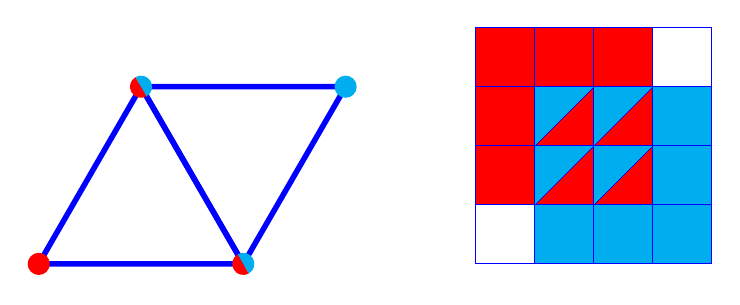
\begin{tikzpicture}
[matrix/.style={rectangle, inner sep = 0, minimum size = 0.75cm, draw =
blue, line width=0, anchor = north east},
element/.style={regular polygon, regular polygon sides=3, draw=blue,
line width=2pt, inner sep=0, outer sep=0, minimum size = 3cm}]

\node (A) [element] at (0,0) {};
\node (B) [element, anchor=corner 1, rotate=180] at
(A.corner 3) {};

\node [circle, fill=red, inner sep = 0, minimum size=8pt] at
(A.corner 2) {};
\node [semicircle, fill=red, line width=0, inner sep = 0, minimum size =4pt, rotate
=120, anchor=south] at
(A.corner 3) {};
\node [semicircle, fill=red, line width=0, inner sep = 0, minimum size =4pt, rotate
=120, anchor=south] at
(A.corner 1) {};


\node [circle, fill=cyan, inner sep=0, minimum size=8pt] at
(B.corner 2) {};
\node [semicircle, fill=cyan, line width=0, inner sep = 0, minimum size =4pt, rotate
=-60, anchor=south] at
(B.corner 3) {};
\node [semicircle, fill=cyan, line width=0, inner sep = 0, minimum size =4pt, rotate
=-60, anchor=south] at
(B.corner 1) {};

\node [matrix]
at (5, 0) {};
\node [matrix, fill=cyan]
at (5.75, 0) {};
\node [matrix, fill=cyan]
at (6.5, 0) {};
\node [matrix, fill=cyan]
at (7.25, 0) {};

\node [matrix, fill=red]
at (5, 0.75) {};
\node (M1) [matrix]
at (5.75, 0.75) {};
\node (M2) [matrix]
at (6.5, 0.75) {};
\node [matrix, fill=cyan]
at (7.25, 0.75) {};

\node [matrix, fill=red]
at (5, 1.5) {};
\node (M3) [matrix]
at (5.75, 1.5) {};
\node (M4) [matrix]
at (6.5, 1.5) {};
\node [matrix, fill=cyan]
at (7.25, 1.5) {};

\foreach \thing in {M1, M2, M3, M4}
{
\draw [fill=cyan, line width=0, draw=blue] (\thing.south west) --
(\thing.north east) -- (\thing.north west) -- cycle;

\draw [fill=red, line width=0, draw=blue] (\thing.south west) --
(\thing.north east) -- (\thing.south east) -- cycle;
}
\node [matrix, fill=red]
at (5, 2.25) {};
\node [matrix, fill=red]
at (5.75, 2.25) {};
\node [matrix, fill=red]
at (6.5, 2.25) {};
\node [matrix]
at (7.25, 2.25) {};

\end{tikzpicture}
\end{center}
\end{frame}

\begin{frame}[label={sec:orgheadline17}]{What do we need for FEM in OP2?}
\begin{itemize}
\item Extensions to OP2 data types
\begin{description}
\item[{\emph{Sparsity}}] the outer product of two Maps
\item[{\emph{Mat}}] Data defined on a sparsity
\end{description}
\item Sum over elements is \emph{par$\backslash$\(_{\text{loop}}\)}
\item insertion into Mat needs to worry about data dependencies
\end{itemize}
\end{frame}

\begin{frame}[fragile,label={sec:orgheadline18}]{What does it look like?}
 \begin{minted}[frame=none,xleftmargin=1em,xrightmargin=1em,fontsize=\scriptsize,mathescape]{python}
par_loop(kernel, elements,
         matrix((elem_node, elem_node), INC),
         node_values(elem_node, READ))
\end{minted}

\begin{itemize}
\item kernel assembles contribution from one element
\begin{itemize}
\item this is N\(_{\text{l}}\) \texttimes{} N\(_{\text{l}}\) dense, N\(_{\text{l}}\) number of dofs in element
\end{itemize}
\item N\(_{\text{l}}\) gets big fast
\begin{itemize}
\item \emph{really} bad for GPUs
\end{itemize}
\end{itemize}
\end{frame}

\begin{frame}[fragile,label={sec:orgheadline19}]{More parallelism}
 \begin{itemize}
\item Expose parallelism within matrix block
\end{itemize}

\begin{minted}[frame=none,xleftmargin=1em,xrightmargin=1em,fontsize=\scriptsize,mathescape]{python}
par_loop(kernel, elements(N_l, N_l),
         matrix((elem_node[i[0]],
                 elem_node[i[1]]), INC),
         node_values(elem_node, READ))
\end{minted}

\begin{itemize}
\item kernel assembles one entry in element matrix
\item runtime has more choice to map to hardware
\begin{itemize}
\item GPU one thread-block per element
\item CPU one thread per element (say)
\end{itemize}
\item can choose different strategies based on size of N\(_{\text{l}}\)
\end{itemize}
\end{frame}

\section{MOAR AUTOMATION}
\label{sec:orgheadline27}

\begin{frame}[label={sec:orgheadline21}]{Writing kernels}
\begin{itemize}
\item By hand
\item use a tool to generate them
\begin{itemize}
\item we've already decided automation is good
\end{itemize}
\end{itemize}
\end{frame}

\begin{frame}[label={sec:orgheadline22}]{Automated generation of FEM code}
\begin{itemize}
\item Most of this comes from FEniCS
\url{http://www.fenicsproject.org}
\item we use their framework (modified) to
\begin{itemize}
\item generate the assembly kernel for FE
\item \ldots{}
\item profit
\end{itemize}
\end{itemize}
\end{frame}

\begin{frame}[label={sec:orgheadline23}]{Writing FE code is \emph{easy}}
\begin{itemize}
\item Let's solve the Poisson equation
\end{itemize}

\begin{align*}
-\nabla^2 u(x, y) &= 0 \;\;\;\;& u \in \Omega\\
u(x, y) &= \sin(2\pi(x + y)) & u \in \partial\Omega
\end{align*}

\begin{description}
\item[{\(\Omega\)}] unit circle
\item[{\(\partial \Omega\)}] outer edge
\end{description}
\end{frame}

\begin{frame}[fragile,label={sec:orgheadline24}]{One slide of code}
 \begin{minted}[frame=none,xleftmargin=1em,xrightmargin=1em,fontsize=\scriptsize,mathescape]{python}
from dolfin import *
mesh = UnitCircle(40)
V = FunctionSpace(mesh, 'CG', 1)
u,v = TrialFunction(V), TestFunction(V)
a = dot(grad(u), grad(v))*dx
L = Constant(0)*v*dx
u0 = Expression('sin((x[0] + x[1])*2*pi)')
def bdry(x, on_boundary):
    return on_boundary
u_h = Function(V)
solve(a == L, u_h, DirichletBC(V, u0, bdry))
plot(u_h, axes=True)
\end{minted}
\end{frame}

\begin{frame}[label={sec:orgheadline25}]{FEM is \emph{easy}}
\begin{itemize}
\item Write down the weak form
\item specify boundary conditions
\item choose your element basis
\item type some python
\item works in parallel too
\end{itemize}
\end{frame}

\begin{frame}[label={sec:orgheadline26}]{So why PyOP2}
\begin{itemize}
\item Not just for FE
\begin{itemize}
\item any unstructured grid computation
\end{itemize}
\item FEniCS have no GPU support
\item we're designing to be embeddable
\begin{itemize}
\item i.e. use \emph{inside} another application
\end{itemize}
\end{itemize}
\end{frame}

\section{Embedding in an existing application}
\label{sec:orgheadline33}
\begin{frame}[label={sec:orgheadline28}]{PyOP2 + Fluidity}
\begin{itemize}
\item Fluidity a general-purpose CFD package
\item to assemble an unsupported equation type
\begin{itemize}
\item write lots of fortran
\item now, write some python
\end{itemize}

\item Works (sort of) now
\begin{itemize}
\item MPI not there yet
\item GPU on its way
\end{itemize}
\end{itemize}
\end{frame}

\begin{frame}[label={sec:orgheadline29}]{Preliminary performance}
\begin{itemize}
\item P1 advection-diffusion
\item single core
\item \textasciitilde{}74000 elements (\textasciitilde{}37000 dofs)
\item 5000 timesteps
\item Fluidity builtin support (\textasciitilde{}2000 loc)
\begin{itemize}
\item \textasciitilde{}7 minutes 40 seconds; assembly + solve \textasciitilde{}400 seconds
\end{itemize}
\item PyOP2 \emph{inside} Fluidity
\begin{itemize}
\item \textasciitilde{}2 minutes 40 seconds; assembly + solve \textasciitilde{}95 seconds
\end{itemize}
\end{itemize}
\end{frame}

\begin{frame}[fragile,label={sec:orgheadline30}]{We can fit the PyOP2 code on a slide}
 \begin{minted}[frame=none,xleftmargin=1em,xrightmargin=1em,fontsize=\scriptsize,mathescape]{python}
t=state.scalar_fields["Tracer"]
u=state.vector_fields["Velocity"]
p=TrialFunction(t)
q=TestFunction(t)
diffusivity = 0.1
M=p*q*dx
adv_rhs = (q*t+dt*dot(grad(q),u)*t)*dx
d=-dt*diffusivity*dot(grad(q),grad(p))*dx
D=M-0.5*d
diff_rhs=action(M+0.5*d,t)
solve(M,t,adv_rhs)
solve(D,t,diff_rhs)
\end{minted}
\end{frame}

\begin{frame}[label={sec:orgheadline31}]{Acknowledgements}
\begin{itemize}
\item OP2
\begin{description}
\item[{Oxford}] Mike Giles, Gihan Mudalige
\item[{Imperial}] Carlo Bertolli, David Ham, Paul Kelly, Florian Rathgeber
\end{description}
\item PyOP2
\begin{description}
\item[{Imperial}] David Ham, Nicolas Loriant, Graham Markall, Florian Rathgeber
\end{description}
\end{itemize}
\end{frame}

\begin{frame}[label={sec:orgheadline32}]{Questions?}
\begin{itemize}
\item comments?
\item anything else?
\end{itemize}
\end{frame}
\end{document}
